%%% LaTeX Template: Two column article
%%%
%%% Source: http://www.howtotex.com/
%%% Feel free to distribute this template, but please keep to referal to http://www.howtotex.com/ here.
%%% Date: February 2011

%%% Preamble
\documentclass[	DIV=calc,%
							paper=a4,%
							fontsize=11pt,
							onecolumn]{scrartcl}	 					% KOMA-article class
\usepackage{amsmath}
\usepackage{algorithm}
\usepackage[noend]{algpseudocode}
\usepackage{graphics,graphicx, float}
\makeatletter
\def\BState{\State\hskip-\ALG@thistlm}
\makeatother
\usepackage{lipsum}													% Package to create dummy text
\usepackage{hyperref}
\usepackage[spanish]{babel}										% English language/hyphenation
\usepackage[protrusion=true,expansion=true]{microtype}				% Better typography
\usepackage{amsmath,amsfonts,amsthm}					% Math packages
%\usepackage[pdftex]{graphicx}									% Enable pdflatex
\usepackage[svgnames]{xcolor}									% Enabling colors by their 'svgnames'
\usepackage[hang, small,labelfont=bf,up,textfont=it,up]{caption}	% Custom captions under/above floats
\usepackage{epstopdf}												% Converts .eps to .pdf
\usepackage{subfig}													% Subfigures
\usepackage{booktabs}												% Nicer tables
\usepackage{fix-cm}													% Custom fontsizes
\usepackage[utf8]{inputenc}

%%% Custom sectioning (sectsty package)
\usepackage{sectsty}													% Custom sectioning (see below)
\allsectionsfont{%															% Change font of al section commands
	\usefont{OT1}{phv}{b}{n}%										% bch-b-n: CharterBT-Bold font
	}

\sectionfont{%																% Change font of \section command
	\usefont{OT1}{phv}{b}{n}%										% bch-b-n: CharterBT-Bold font
	}



%%% Headers and footers
\usepackage{fancyhdr}												% Needed to define custom headers/footers
	\pagestyle{fancy}														% Enabling the custom headers/footers
\usepackage{lastpage}

% Header (empty)
\lhead{}
\chead{}
\rhead{}
% Footer (you may change this to your own needs)
\lfoot{\footnotesize \texttt{HowToTeX.com} \textbullet ~Metaheurísticas \textbullet ~ Curso 2015-2016}
\cfoot{}
\rfoot{\footnotesize page \thepage\ of \pageref{LastPage}}	% "Page 1 of 2"
\renewcommand{\headrulewidth}{0.0pt}
\renewcommand{\footrulewidth}{0.4pt}



%%% Creating an initial of the very first character of the content
\usepackage{lettrine}
\newcommand{\initial}[1]{%
     \lettrine[lines=3,lhang=0.3,nindent=0em]{
     				\color{DarkGoldenrod}
     				{\textsf{#1}}}{}}



%%% Title, author and date metadata
\usepackage{titling}															% For custom titles

\newcommand{\HorRule}{\color{DarkGoldenrod}%			% Creating a horizontal rule
									  	\rule{\linewidth}{1pt}%
										}

\pretitle{\vspace{-30pt} \begin{flushleft} \HorRule
				\fontsize{40}{40} \usefont{OT1}{phv}{b}{n} \color{DarkRed} \selectfont
				}
\title{Búsquedas Híbridas para el Problema
de la Selección de Características}	% Title of your article goes here
\posttitle{\par\end{flushleft}\vskip 0.5em}

\preauthor{\begin{flushleft}
					\large \lineskip 0.5em \usefont{OT1}{phv}{b}{sl} \color{DarkRed}}
\author{Mª Cristina Heredia Gómez, }											% Author name goes here
\postauthor{\footnotesize \usefont{OT1}{phv}{m}{sl} \color{Black}
					Metaheurísticas, Universidad de Granada 								% Institution of author
					\par\end{flushleft}\HorRule}

\date{}																				% No date



%%% Begin document
\begin{document}
\maketitle
\thispagestyle{fancy} 			% Enabling the custom headers/footers for the first page
% The first character should be within \initial{}
\initial{E}\textbf{n esta práctica se estudia el funcionamiento de Algoritmos Meméticos, y su aplicación en el problema de la selección de características, para lo que se construyen tres variantes de algoritmo híbrido (Genético + Búsqueda Local) que se comparan con Greedy y 3nn. }

\section*{Descripción del problema}
El problema de la selección de características, consiste en seleccionar aquellas características de una base de datos dada que resulten las más representativas, de forma que dicha selección nos permita maximizar la tasa de acierto test de un clasificador.

En estas prácticas tomamos un clasificador Knn con k=3 como función objetivo, por lo que buscamos maximizar la tasa de acierto de clasificación, aplicando metaheurísticas que nos ayuden a elegir correctamente que características seleccionar en cada base de datos. \newline
KNN es un clasificador sencillo basado en distancias, concretamente , con k=3 tenemos en cuenta el voto de los 3 vecinos más cercanos para decidir la clase de un dato dado.

Por lo tanto, nuestra función a maximizar es:

\[tasa class=100\cdot \frac{nº instancias\_bien\_clasificadas}{nº total\_instancias}\]

donde las características se codifican de forma binaria para ser representadas en el problema(1 representa seleccionada/ 0 representa no seleccionada). Para realizar los experimentos se han trabajado con tres bases de datos:

\begin{itemize}
	\item Wdbc (Wisconsin Database Breast Cancer)
	\item Movement\_Libras
	\item Arrhythmia
\end{itemize}
de diferentes tamaños.

\section*{Representación del problema}
En este problema las soluciones se representan como un vector de ceros y unos, que tendrán la longitud del número de columnas de la base de datos considerada en ese momento, menos uno (menos la clase). \newline
Así pues una posible solución sería s=(0110...00) donde 0 significa que la característica i-ésima de la base de datos no se selecciona y 1 lo contrario. \newline
\newline
La \textbf{función objetivo} consiste en maximizar la tasa de clasificación mostrada anteriormente. Para ello, \textbf{se parte de una solución inicial} que será generada aleatoriamente en todos los casos (excepto en el Greedy que parte de una solución vacía, con todas las características a 0) y se tratará, a lo largo de la ejecución del algoritmo, de mejorar esa solución. \newline

Para esto es fundamental a lo largo de la práctica, el uso de tres funciones: la que genera una solución vecina a partir de una solución dada, siguiendo un \textbf{esquema de inversión a nivel de bits}

\begin{algorithm}[H]
\caption{flip}\label{euclid}
\begin{algorithmic}
\Procedure{Flip(solucion,index)}{}
\If {$\text{solucion[index]} == \text{1}$} 
\State $\text{solucion$[\text{index}]$} \gets 0$
\Else \State $\text{solucion$[\text{index}]$} \gets 1$
\EndIf

\EndProcedure


\Return solucion

\end{algorithmic}
\end{algorithm}

Esta función llamada \textbf{flip} recibe como argumento una solución de 0 y 1, y un índice, que es la posición del vector en la que deseamos cambiar el bit, y realiza la inversión del bit presente en dicha posición. \newline

Otra función clave es \textbf{getFeaturesForm} que recibe como argumentos un vector de ceros y unos y una base de datos, y devuelve una fómula compuesta por los nombres de las características de la base de datos especificada que están a 1 en el vector. Devuelve una fórmula con forma:
\[class \sim feature_{1}+feature_{2}+...+feature_{n}\]
que posteriormente se la pasaremos al clasificador.

\begin{algorithm}[H]
\caption{getFeaturesForm}\label{euclid}
\begin{algorithmic}
\Procedure{getFeaturesForm(selected,dataset)}{}
\State $\text{names} \gets 0$
\State $\text{featuresList} \gets 0$
\State $\text{i} \gets 0$
\State $\text{formula} \gets 0$
\State $\text{names} \gets \text{obtener nombres de las columnas del dataset}$
\State
\BState \text{loop}: \text{for i in selected} \text{(itera sobre selected)}
 \If {$\text{selected[i]}==1$}
\State $\text{featuresList} \gets \text{names[i]}$ \text{(mete nombre en la lista)}
\BState \text{end loop}
\State $\text{formula} \gets \text{paste(class,$\sim$,featuresList,separador='+')}$\text{(componer formula)}


\EndIf

\EndProcedure

\BState \Return formula

\end{algorithmic}
\end{algorithm}

La última función, \textbf{Adjust3nn} es la que se invoca para ajustar el modelo usando el clasificador 3NN. Recibe como argumentos una fórmula como la mencionada anteriormente y los datos de training de donde tomará las características indicadas en la fórmula, y devuelve el modelo ajustado con los datos de train. \newline
Para poder hacerlo más modular puse la clase de todos los datasets al final de estos y las nombré como \textbf{class} en los tres conjuntos de datos.


\begin{algorithm}[H]
\caption{Adjust3nn}\label{euclid}
\begin{algorithmic}
\Procedure{Adjust3nn(formula,training data)}{}
\State $\text{modelo} \gets 0$ \text{(inicialmente modelo no contiene nada)}

\State modelo $\gets$ \text{ajusta modelo(formula,training data)}

\EndProcedure

\BState \Return modelo

\end{algorithmic}
\end{algorithm}


Para ajustar el modelo en el código uso el método \textbf{train} de la librería \textbf{caret}. \newline Para calcular las predicciones y el acierto de test uso \textbf{predict} y \textbf{postResample}, también de esta librería. \newline

En esta práctica, he creado una función fusionando las dos anteriores en una, pues la función fitness que recibe la función \textbf{ga(..)} empleada solo puede recibir un vector binario como único argumento. Unifico por tanto las dos funciones anteriores en una:
\begin{algorithm}[H]
\caption{myfitness}\label{euclid}
\begin{algorithmic}
\Procedure{myfitness(selected)}{}
\State $\text{names} \gets 0$
\State $\text{featuresList} \gets 0$
\State $\text{i} \gets 0$
\State $\text{formula} \gets 0$
\State $\text{names} \gets \text{obtener nombres de las columnas del dataset}$
\State $\text{evalua} \gets 0$
\State
\BState \text{loop}: \text{for i in selected} \text{(itera sobre selected)}
 \If {$\text{selected[i]}==1$}
\State $\text{featuresList} \gets \text{names[i]}$ \text{(mete nombre en la lista)}
\BState \text{end loop}
\State
\State $\text{formula} \gets \text{paste(class,$\sim$,featuresList,separador='+')}$\text{(componer formula)}

\State $\text{modelo} \gets 0$ \text{(inicialmente modelo no contiene nada)}

\State modelo $\gets$ \text{ajusta modelo(formula,training data)}
\State \text{evalua} $\gets$ \text{acierto test (modelo)}
\State

\BState \Return evalua

\EndIf

\EndProcedure



\end{algorithmic}
\end{algorithm}

\section*{Algoritmos Meméticos estudiados en esta práctica}


\section*{AM-(10,0.1)}
Se implementa un genético estacionario con una población de 10 cromosomas, y cada 10 generaciones se aplica Búsqueda Local sobre un subconjunto aleatorio de cromosomas con probabilidad = 0.1 para cada cromosoma. \newline
\newline
Las probabilidades de cruce y mutación son 0.7 y 0.001 respectivamente. El algoritmo se detiene cuando realiza 15000 evaluaciones de la función objetivo, o cuando lleva 500 iteraciones sin mejorar la mejor solución actual. Esta segunda condición la he añadido con el objetivo de acortar el tiempo de ejecución, suponiendo que si en 500 ejecuciones no ha mejorado es porque la búsqueda se estanca, bien porque llega al óptimo, bien por otra razón. \newline
Para el genético, la población inicial se genera de forma aleatoria, y se implementa un esquema generacional con elitismo donde en cada generación se conserva la mejor solución generada,sustituyendo a la peor de la población. \newline
El \textbf{operador de selección} empleado es el de torneo binario. El \textbf{operador de cruce}
que se emplea es el de cruce uniforme, donde los bits se copian aleatoriamente del primer o del segundo padre:
\begin{figure}[H] %con el [H] le obligamos a situar aquí la figura
\centering
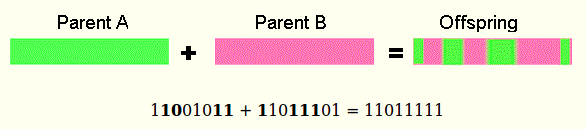
\includegraphics[scale=0.52]{cruce.png}  %el parámetro scale permite agrandar o %achicar la imagen. En el nombre de archivo puede especificar directorios
\label{}
\caption{Operador de cruce uniforme}   
\end{figure}

El \textbf{operador de mutación} empleado es el de mutación aleatoria uniforme, por lo que se toma un bit aleatoriamente y se invierte. 


Pseudocódigo del algoritmo Memético:
\begin{algorithm}[H]
\caption{Algoritmo Memético}\label{euclid}
\begin{algorithmic}
\Procedure{AM(tamPop,presion)}{}
\State $\text{popSize}$ $\gets \text{tamPop}$
\State $\text{pressel}$ $\gets \text{presion}$
\State $\text{nBits}$ $\gets \text{ncol(dataset)-1}$
\State $\text{population}$ $\gets \text{generar Poblacion Aleatoria}$
\State $\text{pcrossover}$ $\gets 0.7$
\State $\text{pmutation}$ $\gets 0.001$
\State $\text{elitism}$ $\gets 0.1$
\State $\text{poptim}$ $\gets 0.1$
\State
\BState \text{loop}: \text{MIENTRAS(no cumpla condición de parada)}
\State
 \State \text{evaluar fitness de cada individuo} 
 \State \text{seleccionar padres por torneo} 
 \State \text{cruzar padres con prob=pcrossover} 
 \State \text{mutar individuo con  prob=pmutation} 
 \State \text{optimizar solucion aplicando BL con prob=poptim y pressel} 
 \State \text{reemplazar población y peor individuo} 
\State
\BState \text{end loop}

\State
\EndProcedure
\end{algorithmic}
\end{algorithm}

El algoritmo recibe como parámetros el tamaño de la población y la presión de selección. De esta forma, con una presión de selección baja, se tienden a seleccionar probilidades prácticamente iguales para cada solución, y por tanto sería como tomarlas aleatoriamente. Para este caso fijo un valor de presión de 0.1. El tamaño de la población es 10 cromosomas. La variable poptim que aparece en la BL es la probabilidad con la que esta se aplica. Como hay que aplicarla cada 10 generaciones, la prob será 0.1.

\section*{AM-(10,0.1*N)}
En este caso se aplicará el mismo Algoritmo Memético de nuevo,aplicando Búsqueda Local cada 10 generaciones, pero esta vez no sobre un subconjunto aleatorio, sino sobre los 0.1$\cdot$N mejores cromosomas de la población actual, donde N es el tamaño de ésta. \newline
El algoritmo es el mismo que el del apartado anterior, y se emplean los mismos operadores y el mismo tamaño de población, sin embargo ahoa se fija la presión de selección a 0.1$\cdot$N, por lo que la BL empezará en una solución seleccionada por su fitness. A más pressión de selección, selecciona soluciones con mayor valor fitness.



\section*{Procedimiento considerado}
En la realización de la práctica he usado lenguaje R y el IDE RStudio,
beneficiándome de las facilidades que R aporta por no ser un lenguaje orientado a objetos ni fuertemente tipado, así como de las potentes librerías de las que dispone. Por otra parte el empleo de R ha supuesto una pérdida en eficiencia. \newline
\newline
Para hacer los Meméticos que se piden, he usado una la librería \textbf{GA} (Genetic Algorithms) cuyo autor es Lucca Scrucca de la Università degli Studi di Perugia, ya que es una librería bastante amplia para genéticos, además de muy configurable, que permite aplicar métodos de optimización/mejora sobre las soluciones obtenidas por el genético, como Búsueda local o enfriamiento simulado.\newline
\newline
El procedimiento a seguir ha sido el siguiente: en primer lugar se realiza la carga de los datos especificando la ruta de los mismos, y luego he realizado un pequeño "preprocesamiento" que consiste en:

\begin{itemize}
\item si hay columnas en los datos con todos los valores iguales, eliminarlas.
\item normalizar los datos, sin normalizar la clase.
\item tomar la columna de la clase y colocarla al final de todas las bases de datos.
\item nombrar igual a las columnas con la clase de los 3 datasets."\textbf{class}", para hacerlo más modular en las funciones. 
\end{itemize}

Una vez listos los datos, he usado, como mencioné arriba, el knn de la librería caret de R, fijando el k a 3, como clasificador y su acierto test como resultado a maximizar.\newline También he usado el método \textbf{createDataPartition} de esta librería, para hacer el particionamiento estratificado de los datos. Parto los datos cada vez con una semilla, que es i$\cdot$9876543, donde i va de 1 a 5(cada interación de CV), y que se replica para cada ejecución de cada algoritmo distinto lanzada con cada base de datos. Luego se intercambian las particiones.\newline El objetivo es que los resultados obtenidos para cada algoritmo sean realmente comparables.\newline
\newline

Para lanzar el memético, la especificación es la siguiente:\newline
$GA<-ga(type = "binary",fitness =myfitness,nBits =ncols, population=gabin_Population,selection=gabin_tourSelection,crossover=gabin_uCrossover,
mutation=gabin_raMutation,                          popSize=10,pcrossover=0.7,pmutation=0.001,elitism=0.1,maxiter=15000,run=500,optim=TRUE,optimArgs = list(method = "L-BFGS-B", poptim = 0.1, pressel =(0.1*N) ,control = list( maxit = 1)))$
\newline

donde: 
\begin{itemize}
\item \textbf{type} es el tipo de codificación del problema
\item \textbf{fitness} es la función fitness a maximizar
\item \textbf{nBits} número de bits de una solución. En este caso ncol(dataset)-1 (le quitamos la clase) 
\item \textbf{population} como generamos la población inicial. En este caso, generamos aleatoriamente cromosomas binarios
\item \textbf{selection} operador de selección. Elegimos \textit{gabin\_tourSelection} que es el torneo binario
\item \textbf{crossover} operador de cruce. Hay varios, seleccionamos el op de cruce binario uniforme
\item \textbf{mutation} operador de mutación. Seleccionamos el binario aleatorio uniforme
\item \textbf{popSize} tamaño de la población
\item \textbf{pcrossover} probabilidad de cruce
\item \textbf{pmutation} probabilidad de mutación
\item \textbf{elitism} número de mejores soluciones que se conservan entre generaciones. Conservamos solo la mejor, luego lo ponemos a 0.1
\item \textbf{maxiter} número máximo de iteracciones antes de que el algoritmo se detenga
\item \textbf{run} máximo de iteracciones consecutivas sin mejora antes de que el algoritmo se detenga. añado esta opción y la pongo a 500 iteracciones porque permite ganar mucho en tiempo de ejecución.
\item \textbf{optim} si se pone a TRUE indica que se va a aplicar método de optimización sobre las soluciones
\item \textbf{optimArgs} lista de argumentos de configuración del método de optimización a aplicar
\item \textbf{method} nombre del método de optimización a aplicar, en este caso, Búsqueda Local primero el mejor
\item \textbf{poptim} probabilidad de ejecutar la Bl en esa iteracción
\item \textbf{pressel} presión de selección 
\item \textbf{control} lista con parámetros de control para la BL como el número de iteracciones a realizar
\end{itemize}

El 5x2 está hecho de forma funcional y se encuentra en la sección de ejecución del algoritmo correspondiente, en el Rscript. Se separan ejecuciones de 5 en 5, en train versus test y test versus train. Las tasas de reducción correspondientes de calculan justo debajo. \newline
%\begin{table}
%\caption{Random table}
%\centering
%	\begin{tabular}{llr}
%		\toprule
%		\multicolumn{2}{c}{Name} \\
%		\cmidrule(r){1-2}
%			First name & Last Name & Grade \\
%		\midrule
%			John & Doe & $7.5$ \\
%			Richard & Miles & $2$ \\
%		\bottomrule
%	\end{tabular}
%\end{table}



El Algoritmo greedy usado como comparativa, es el usado en prácticas anteriores, que en pseudocódigo se puede definir como:
\begin{algorithm}[H]
\caption{greedyRndm}\label{euclid}
\begin{algorithmic}
\Procedure{greedyRndm(training,test,seed)}{}
\State $\text{featuresList} \gets \text{lista de caracteristicas del dataset}$
\State $\text{final} \gets \text{FALSE}$
\State \text{selectedAndCandidate} $\gets 0 $ \text{(inicialmente no hay seleccionadas)}
\State \text{ganancias} $\gets 0 $ \text{(inicialmente está vacía)}
\State \text{selected} $\gets 0 $ \text{(inicialmente está vacía)}
\State $\text{cmejor} \gets \text{0}$
\State $\text{cpeor} \gets \text{0}$
\State $\text{umbral} \gets \text{0}$
\State $\text{alpha} \gets \text{0.3}$
\State $\text{randomFeature} \gets \text{0}$
\State $\text{evalua} \gets \text{0}$
\State $\text{bestAccu} \gets \text{0}$ \text{(mejor acierto test hasta ahora)}
\State \text{LRC} $\gets 0 $ \text{(inicialmente está vacía)}

\State
\BState \text{loop}: \text{mientras(featuresList!=0 AND !final )}
\State $\text{ganancias}$ $\gets $\text{calcular ganancia test de cada caracteristica por separado}
\State $\text{cmejor}$ $\gets $\text{max(ganancias)}
\State $\text{cpeor}$ $\gets $\text{min(ganancias)}
\State $\text{umbral} \gets $\text{cmejor-(alpha(cmjor-cpeor))} 
\State $\text{LRC} \gets $\text{caracteristicas cuyas (ganancias$>=$umbral)} 
\State $\text{randomFeature} \gets \text{caracteristica alatoria de LRC}$
\State $\text{selectedAndCandidate[randomFeature]} \gets 1$
\State $\text{evalua} \gets \text{ajustar de nuevo usando las caracteristicas de selectedAndCandidate }$
\State
\If{\text{evalua} $>$ \text{bestAccu}} 
\State \text{bestAccu} $\gets$ \text{evalua}
\State \text{selected} $\gets$ \text{selectedAndCandidate}
\State \text{featuresList[randomFeature]} $\gets$ \text{no se puede volver a seleccionar}
\State
\Else{ \text{final} $\gets$ \text{TRUE}}

\EndIf
\State

\BState $\text{selectedAndCandidate} \gets \text{selected}$
\State
\BState \text{end loop}

\EndProcedure

\BState \Return list(selected,bestAccu)

\end{algorithmic}
\end{algorithm}

\section*{Análisis de los resultados}

Se observa en las tablas de resultados(ver resultados\_tablas.ods) que el algoritmo híbrido da los mejores resultados para este problema. Aunque solo se compare con Greedy y 3nn, en otras prácticas se han probado otros algoritmos y este es, sin duda, el que mejores resultados da en estas bases de datos. \newline
\newline
Greedy obtiene un resultado algo superior que el Memético que aplica Bl sobre un subconjunto  aleatorio de cromosomas, pero inferior para el resto de casos de estudio.\newline
\textbf{En cuanto a los tiempos de ejecución} Greedy al tener menos cómputo es el que menos tarda. Le sigue AM(10,0.1) que tarda menos que AM(10,0.1$\cdot$N) debido a la selección aleatoria de cromosomas con prob=0.1, ya que evita tener que buscar los 0.1N mejores.
\newline
\newline
\textbf{En cuanto a la calidad de los resultados} 
El mejor algoritmo en términos de calidad, al menos para las bases de datos chica y mediana, parece que es el memético que aplica BL sobre las mejores soluciones, pues obtiene en media las mejore marcas de aciertos en test. Sin embargo, no es así para el caso de Arritmia, donde observamos que obtiene peores resultados en calidad que la otra versión de AM implementado e incluso que Greedy. Aunque esto puede deberse en parte a la población inicial, pues he observado que en las 5 particiones parte de una población inicial mala y además se estanca pronto la búsqueda. \newline

En cuanto a las tasas de reducción, se observa que ambos meméticos seleccionan cerca de la mitad de características que selecciona greedy y superan sus resultados en media por lo que muchas de las características que selecicona greedy son prescindibles.\newline
\newline
A pesar de que los resultados no son malos, creo que se podrían mejorar ajustando mejor los parámetros. Se podría intentar elevando el grado de elitismo (ahora mismo sólo se conserva la mejor solución entre poblaciones) y aplicando BL con más probabilidad o más interacciones , o incluso cambiando la BL por otro método de optimización como S.Annealing. En calquier caso, con los ajustes actuales ganamos en tiempo. \newline
He observado que las búsquedas siempre se estancan antes de las 15000 evaluaciones, por lo que, como mencioné arriba, he incorporado una segunda condición para que si el algoritmo lleva sin mejorar la mejor solución 500 iteraciones, se detenga, ahorrando así en tiempo y cómputo. 
\subsection*{Ilustración de resultados}

\begin{figure}[H] %con el [H] le obligamos a situar aquí la figura
\centering
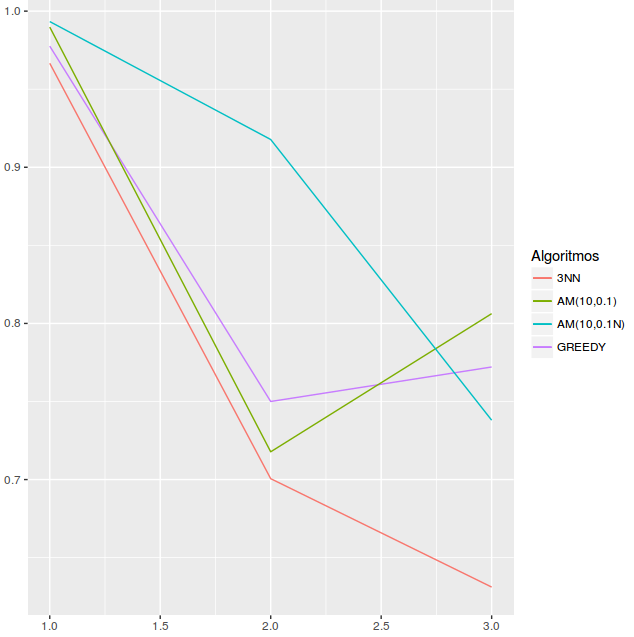
\includegraphics[scale=0.55]{comparativa.png}  %el parámetro scale permite agrandar o %achicar la imagen. En el nombre de archivo puede especificar directorios
\label{}
\caption{Comparativa global de rendimiento }   
\end{figure}
Donde en el eje y se representa de 0 a 1 el \% de clasificación test obtenido, y en el eje X,tenemos : 
\begin{itemize}
\item 1 : representa WDBC
\item 2 : representa Movement Libras
\item 3 : representa Arritmia
\end{itemize}

\section*{Referencias}
\url{https://cran.r-project.org/web/packages/GA/GA.pdf}
\url{https://github.com/luca-scr/GA/blob/master/R/ga.R}
\end{document}
